\documentclass[final]{beamer}

% ====================
% Packages
% ====================

\usepackage[T1]{fontenc}
\usepackage{lmodern}
\usepackage[size=custom,width=120,height=72,scale=1.0]{beamerposter}
\usetheme{gemini}
\usecolortheme{gemini}
\usepackage{graphicx}
\usepackage{booktabs}
\usepackage{tikz}
\usepackage{xcolor}
\usepackage{pgfplots}
\pgfplotsset{compat=1.7}

% ====================
% Lengths
% ====================

% If you have N columns, choose \sepwidth and \colwidth such that
% (N+1)*\sepwidth + N*\colwidth = \paperwidth
\newlength{\sepwidth}
\newlength{\colwidth}
\setlength{\sepwidth}{0.025\paperwidth}
\setlength{\colwidth}{0.3\paperwidth}

\newcommand{\separatorcolumn}{\begin{column}{\sepwidth}\end{column}}

% ====================
% Title
% ====================

\title{SINGLE-PARTICLE MOTION IN A WOBBLING NUCLEUS \\ A CASE-STUDY FOR ODD-MASS ISOTOPES}

\author{Robert Poenaru \inst{1,2} | \texttt{robert.poenaru@protonmail.ch}}

%\institute[shortinst]{\inst{1} Doctoral School of Physics, University of Bucharest, Bucharest, Romania \samelineand \inst{2} Department of Theoretical Physics, Horia-Hulubei National Institute of Nuclear Physics and Engineering, Bucharest-Magurele, Romania}

\institute[shortinst]{\inst{1} Doctoral School of Physics, University of Bucharest, Bucharest, Romania \\ \inst{2} Department of Theoretical Physics, Horia-Hulubei National Institute of Nuclear Physics and Engineering, Bucharest-Magurele, Romania}

% ====================
% Body
% ====================

\begin{document}

\addtobeamertemplate{headline}{} 
{\begin{tikzpicture}[remember picture, overlay]
     \node [anchor=north east, inner sep=0.9cm]  at (current page.north east)
     {
\includegraphics[height=11cm]{./images/logo.png}};
     \node [anchor=north west, inner sep=0.9cm]  at (current page.north west)
     {
\includegraphics[height=11cm]{./images/uniLogo.png}};
  \end{tikzpicture}}


\begin{frame}[t]
\begin{columns}[t]
\separatorcolumn

\begin{column}{\colwidth}

  \begin{block}{Introduction}

Triaxial nuclei are nuclear objects which have an asymmetry between the moments of inertia associated with the principal axes of the ellipsoid and, therefore, a triaxial nucleus has an asymmetry in the mass/charge distributions within the nucleus. This \emph{feature} gives rise to rich energy spectra of collective character, and interactions between different states of predominately electric $E2$ type.

In the present work, a description of the collective motion which occurs in strongly-deformed odd-mass triaxial nuclei known as \emph{Wobbling Motion} (WM) is done, using the \emph{Particle Rotor Model} (PRM) \cite{bohr1998nuclear}. Within this framework, the total nuclear system consists of an even-even core and a \emph{valence} nucleon (also known as \emph{intruder}) which is moving in a quadrupole deformed mean field, generated by the core.

The strength of the deformed potential in which the odd single-particle is confined turns out to be a major player in the description of the wobbling spectrum of a nucleus, since different coupling strengths between the core and the intruder nucleon will lead to different rotational spectra, or even transition probabilities.

By adopting a deformed potential of Nilsson type \cite{nilsson1955mat} in the expression of the total Hamiltonian that describes an odd-$A$ triaxial nucleus, it is possible to describe the energy spectrum of several isotopes in which wobbling motion is known to occur. The coupling parameter that enters in the expression of the deformed potential (\emph{single-particle Hamiltonian}) depends on the deformation parameters of the nuclear shapes is expressed in several ways, and a quantitative comparison between all of them is made.

  \end{block}

  \begin{block}{Wobbling Motion}
  
\begin{itemize}
    \item The wobbling phenomenon in nuclei implies a \emph{precession} of the total angular momentum combined with an \emph{oscillation} of its projection onto the rotation axis.
    \item Triaxial nuclei are objects with all three moments of inertia associated with the principal axes different in magnitude, making it possible for rotation to occur around all three axes. This results in a rich rotational spectrum with a collective character.
\end{itemize}
  \end{block}
 

\end{column}

\separatorcolumn

\begin{column}{\colwidth}

\begin{figure}
      \centering
      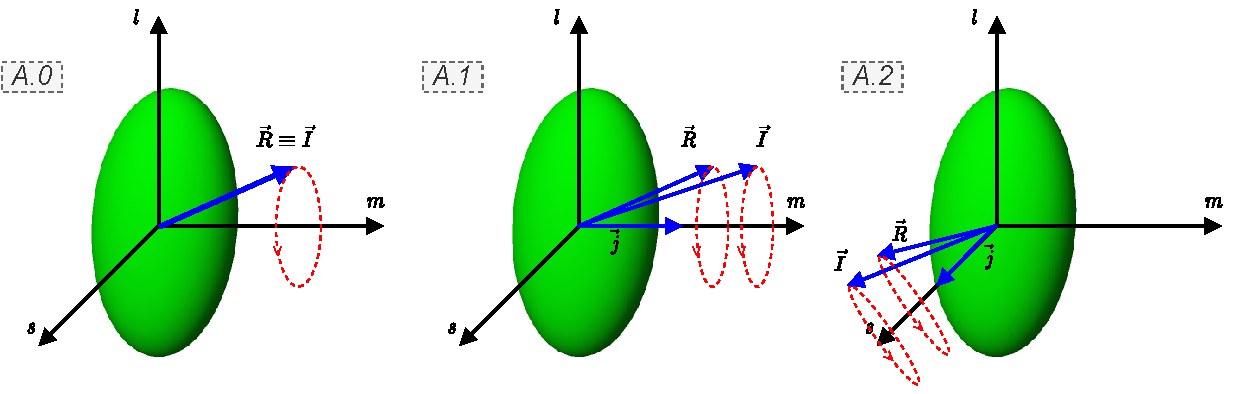
\includegraphics[scale=1.55]{images/wobbling_Regimes_COUPLING_SCHEME.pdf}
      \caption{An illustration with the wobbling regimes which can occur in a nucleus.}
      \label{wobbling-regimes}
  \end{figure}


    \begin{block}{Wobbling Motion - Odd-A Case}
 \begin{figure}
\centering
\begin{minipage}{.5\textwidth}
  \centering
  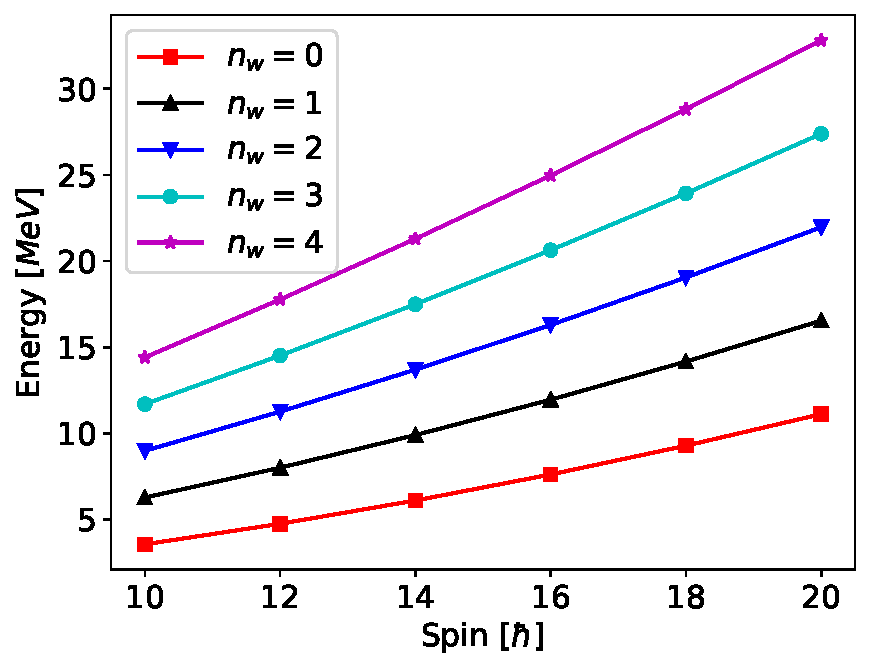
\includegraphics[scale=0.8]{images/simple_wobbling_spectrum.pdf}
\end{minipage}%
\begin{minipage}{.5\textwidth}
  \centering
 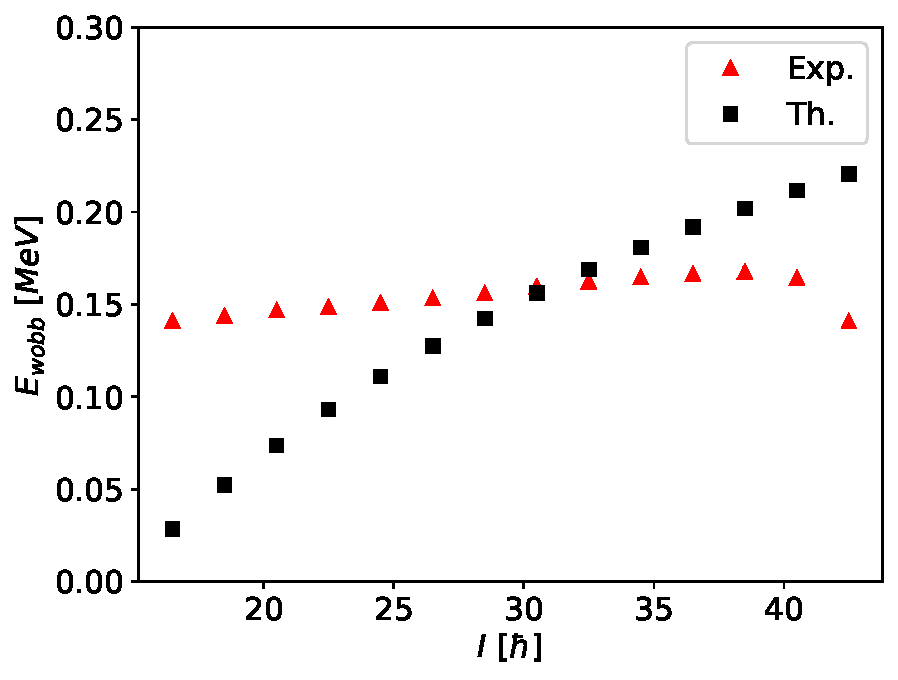
\includegraphics[scale=0.8]{images/wobbling_energy_ThExp.pdf}
\end{minipage}
\caption{The energy function $\mathcal{H}$, evaluated in one of its minimum points, as a function of the polar coordinates. One coordinate is fixed while the other one is varied within its interval of existence. For $\theta\in[0,\pi]$ and $\varphi\in[0,2\pi]$. The chosen minimum is $p_\text{min}=\left(\frac{\pi}{2},0\right)$. Each spin state corresponds to one of the four triaxial bands of $^{163}$Lu.}
    \label{energy-function-min-point-evolution}
\end{figure}
  \end{block}

  \begin{block}{Single-Particle Deformed Potential}

  \end{block}
  
\end{column}

\separatorcolumn

\begin{column}{\colwidth}

  \begin{block}{A block containing some math}

    \heading{A heading inside a block}
  One.

    \heading{Another heading inside a block}
 One.

  \end{block}

  \begin{block}{Results}
    Some results.
    \begin{table}
      \centering
      \begin{tabular}{l r r c}
        \toprule
        \textbf{First column} & \textbf{Second column} & \textbf{Third column} & \textbf{Fourth} \\
        \midrule
        Foo & 13.37 & 384,394 & \alpha \\
        Bar & 2.17 & 1,392 & \beta \\
        Baz & 3.14 & 83,742 & \delta \\
        Qux & 7.59 & 974 & \gamma \\
        \bottomrule
      \end{tabular}
      \caption{A table caption.}
    \end{table}
  \end{block}
  
    \begin{block}{Conclusions}
    Some conclusions.
    \begin{table}
      \centering
      \begin{tabular}{l r r c}
        \toprule
        \textbf{First column} & \textbf{Second column} & \textbf{Third column} & \textbf{Fourth} \\
        \midrule
        Foo & 13.37 & 384,394 & \alpha \\
        Bar & 2.17 & 1,392 & \beta \\
        Baz & 3.14 & 83,742 & \delta \\
        Qux & 7.59 & 974 & \gamma \\
        \bottomrule
      \end{tabular}
      \caption{A table caption.}
    \end{table}
  \end{block}

  \begin{block}{References}

    \nocite{*}
    \footnotesize{\bibliographystyle{plain}\bibliography{poster}}

  \end{block}

\end{column}

\separatorcolumn

\end{columns}

\end{frame}

\end{document}